\section{Correlations with Sea Ice Extent}
In light of work done by other researchers which looked at global temperature correlated with the total amount of sea ice in Antarctica. \cite{Wang2019Compounding2016, Meehl2019Sustained2016} we carried out this comparison ourselves. Taking the Pearson correlation between the time series of 2m temperature at each gridpoint globally with the time series of total sea ice in Antarctica. \textcolor{red}{I'm not sure of the legitimacy of the above paragraph.}

In computing the correlations with SIE in Antarctica, we would expect the largest signal to come from seasonal variations in the different variables. This means that we are expecting large positive and negative correlations for each variable we are looking at, with spatial structures which should give us some physical understanding of how each variable acts in relation to the amount of sea ice around Antarctica.

% \begin{figure}[H]
%     \centering
%     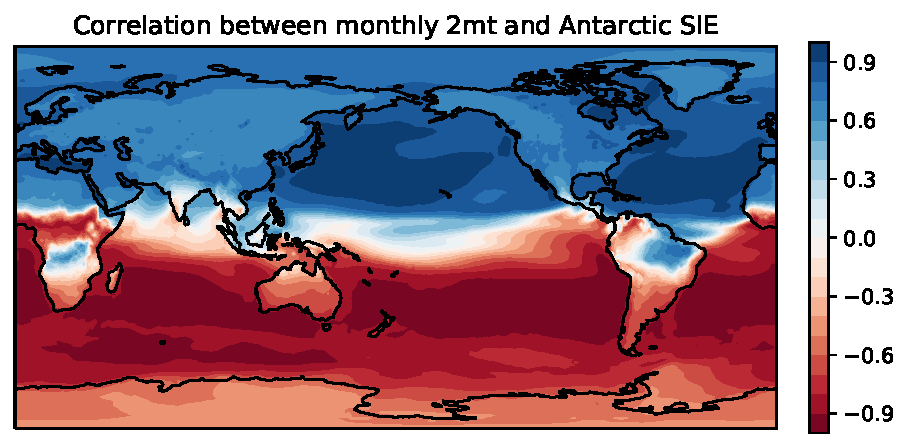
\includegraphics[width=\textwidth]{Images/global_correlation_m2mt_sie.pdf}
%     \caption{Correlation between monthly averaged 2m temperature and total SIE in Antarctica.}
%     \label{fig:my_label}
% \end{figure}

% I haven't done any preprocessing with this data so far. I believe the papers looked at some kind of anomaly in the amount of sea ice, as such I will look into doing something similar next week.
% What we see here however is good as we see a positive correlation in the northern hemisphere and a negative correlation in the southern hemisphere.

% \begin{figure}[H]
%     \centering
%     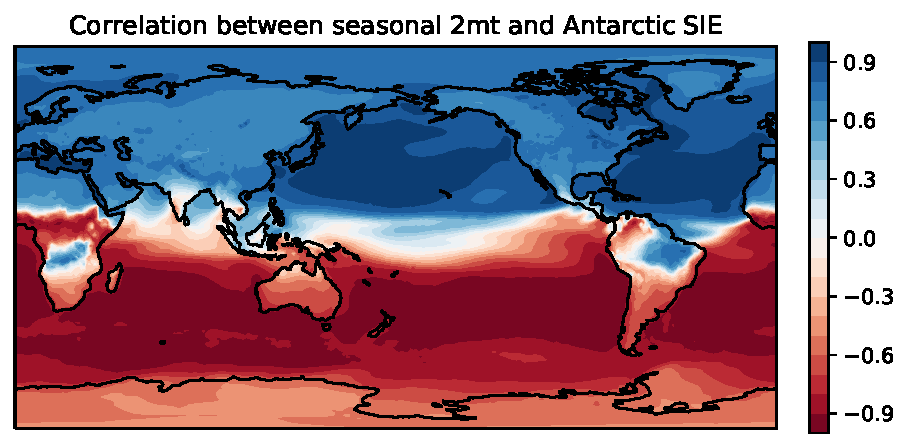
\includegraphics[width=\textwidth]{Images/global_correlation_s2mt_sie.pdf}
%     \caption{Correlation between seasonally averaged 2m temperature and total SIE in Antarctica.}
%     \label{fig:my_label}
% \end{figure}
% We note no difference between the monthly and seasonal correlations between the two datasets. This is good as we would not expect to see a large difference.


\begin{figure}[H]
    \centering
    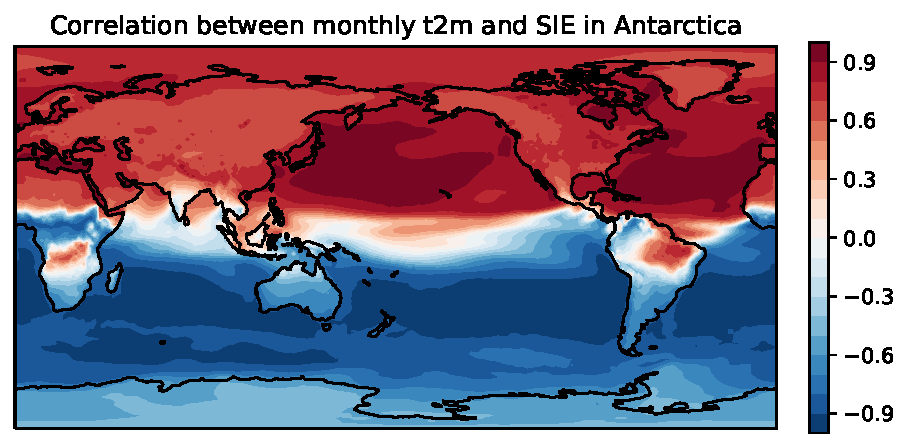
\includegraphics[width=\textwidth]{Images/global_correlation_monthly_t2m_sie.pdf}
    \caption{Correlation between 2m temperature globally and total Sea Ice Extent in Antarctica.}
    \label{fig:temp_sie_corr}
\end{figure}

We note that there is a strong seasonal signal present here. This results in the temperatures in the northern hemisphere being positively correlated with the extent of Antarctic ice. We see a corresponding negative correlation in the southern hemisphere.

We ran the same calculation also for pressure and wind speeds. The results of which are included below.
\begin{figure}[H]
    \centering
    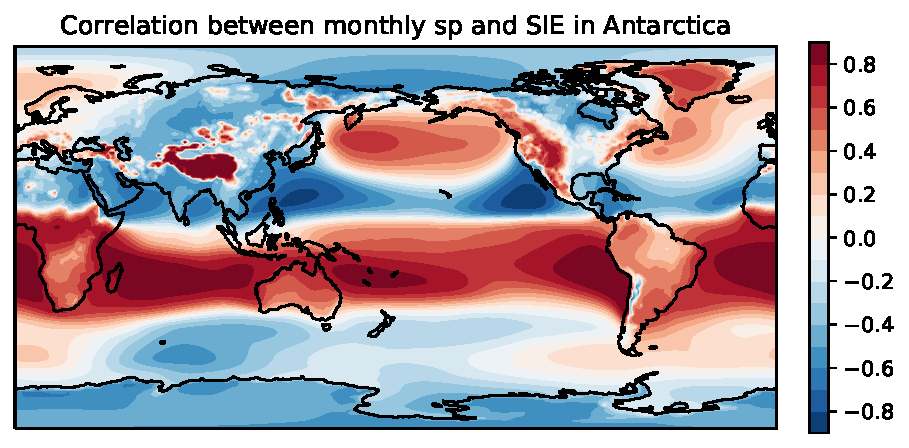
\includegraphics[width=\textwidth]{Images/global_correlation_monthly_sp_sie.pdf}
    \caption{Correlation between surface pressure globally and total Sea Ice Extent in Antarctica.}
    \label{fig:sp_sie_corr}
\end{figure}
We note that the pressure seems to be broken up longitudinally, with a negative correlation near the sea ice followed by a strong positive correlation in the tropics, another negative correlation and then a positive correlation. \textcolor{red}{Possibly because of atmospheric structure? or SAM? Explore.} Also of note is the discrepancies over land in the northern Hemisphere. \textcolor{red}{Maybe Explore?}


\begin{figure}[H]
    \centering
    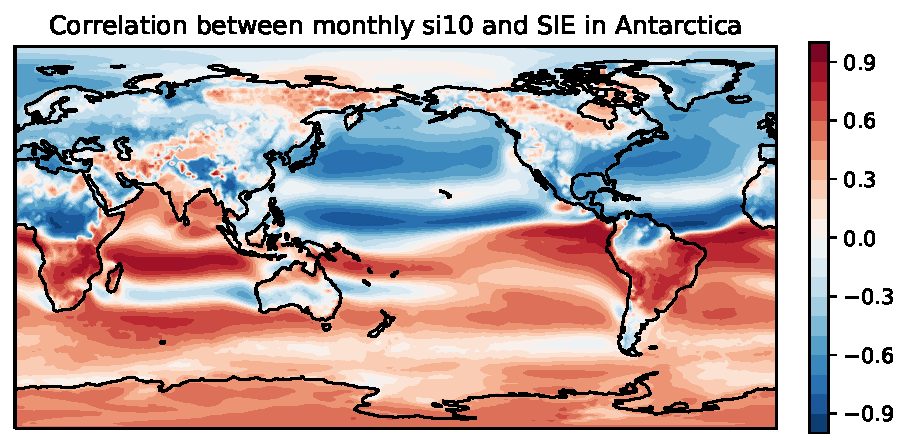
\includegraphics[width=\textwidth]{Images/global_correlation_monthly_si10_sie.pdf}
    \caption{Correlation between 10m wind speed globally and total Sea Ice Extent in Antarctica.}
    \label{fig:si10_sie_corr}
\end{figure}

The total wind speed seems generally split similarly to the temperature correlations, broken up into the northern and southern hemispheres. With generally positive correlations in the southern hemisphere and negative correlations in the northern hemisphere. This indicates potentially a strong seasonal signal which we can explore further by looking at the correlations between SIE and the u and v wind components.

\begin{figure}[H]
    \centering
    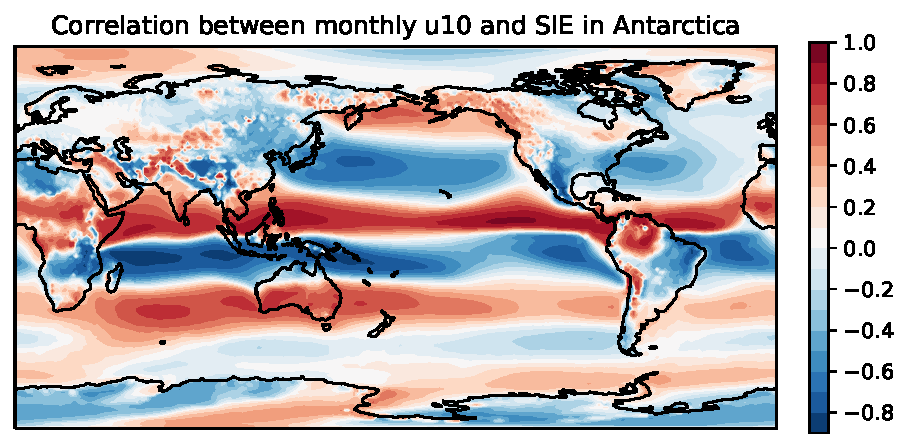
\includegraphics[width=\textwidth]{Images/global_correlation_monthly_u10_sie.pdf}
    \caption{Correlation between u component 10m wind speed globally and total Sea Ice Extent in Antarctica.}
    \label{fig:u10_sie_corr}
\end{figure}

I don't yet have a physical explanation for the bands we see here, but a structure is clearly there and worth discussing. Maybe ENSO?

\begin{figure}[H]
    \centering
    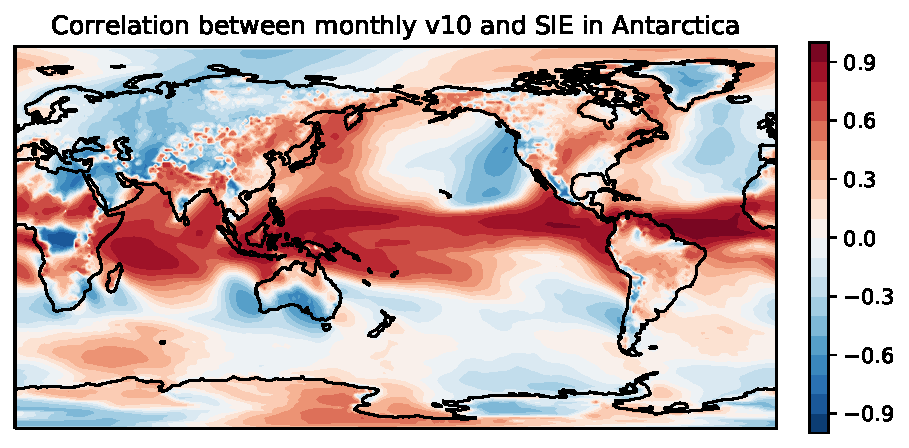
\includegraphics[width=\textwidth]{Images/global_correlation_monthly_v10_sie.pdf}
    \caption{Correlation between v component 10m wind speed globally and total Sea Ice Extent in Antarctica.}
    \label{fig:v10_sie_corr}
\end{figure}

I don't yet have a physical explanation for the bands we see here, but a structure is clearly there and worth discussing.

As expected the largest signal we are seeing in most of these plots is a seasonal one. This makes sense as the seasons are some of the largest climate drivers in the atmosphere and ocean.